\documentclass[12pt]{article}

\usepackage{../discrete}
\usetikzlibrary{shapes,snakes}
\usepackage{pgf}

\heading{Math 228}{}{Counting Notes}



\begin{document}

One of the first things you learn in mathematics is how to count.  Now we are going to learn that all over again, and you will find that counting is a lot harder than you remember.  The problem is that we want to count large collections of things quickly and precisely.  For example:
\begin{itemize}
 \item How many different lotto tickets are possible?
 \item In a group of 10 people, if everyone shakes hands with everyone else exactly once, how many handshakes took place?\footnote{We know the answer to this thanks to graph theory - we are asking how many edges there are in $K_{10}$.  What if your group had a secrete 3-person handshake?  If every group of three people participated in such a handshake, how many handshakes take place?  Equivalently, how many triangles are there in $K_{10}$?}
 \item How many ways can you distribute 10 girl scout cookies to 7 boy scouts?
 \item How many 10 digit numbers contain exactly 4 prime digits?
 \item How many functions $f: \{1,2,3,4\} \to \{1,2,3\}$ are onto?  
 \item How many subsets of $\{1,2,3,\ldots, 10\}$ have cardinality 7?
\end{itemize}

Before tackling these difficult questions, let's look at the basics of counting.

\section{Additive and Multiplicative Principles}

Consider this rather simple counting problem: at Red Dogs and Donuts, there are 14 varieties of donuts, and 16 types of hot-dogs.  If you want either a donut or a dog, how many options do you have?  This is an easy question - you just add 14 and 16.  Will that always work?  What is important here?


\begin{defbox}{Additive Principle}
  The {\em additive principle} states that if an event $A$ can occur in $m$ ways, and event $B$ can occur in $n$ {\em disjoint} ways, then the event ``$A$ or $B$'' can occur in $m + n$ ways.  
\end{defbox}

It is important that the events be disjoint.  For example, a standard deck of 52 cards contains $26$ red cards and $12$ face cards.  However, the number of ways to select a card which is either red or a face card is not $26 + 12 = 38$.  This is because there are 6 cards which are both red and face cards.

The additive principle works with more than two events.  Say you would also consider eating one of 15 waffles?  How many choices do you have now?  You would have $14 + 16 + 15 = 45$ options.

\begin{example}
  How many two letter ``words'' start with either A or B?  How many start with one of the 5 vowels?  (A word is just a strings of letters - they don't have to be English words, or even pronounceable).
  
  \begin{solution}
    First, how many two letter words start with A?  We just need to select the second letter, which can be accomplished in 26 ways.  So there are 26 words starting with A.  There are also 26 words that start with B.  So to select a word which starts with either A or B, we can pick the word from the first 26 or the second 26, for a total of 52 words.  The additive principle is at work here.
    
    Now what about all the two letter words starting with a vowel?  Well there are 26 starting with A, another 26 starting with E, and so on.  We will have 5 groups of 26.  So we add 26 to itself 5 times.  Of course it would be easier to just multiply $5\cdot 26$ - we are really using the additive principle again, just using multiplication as a shortcut.
  \end{solution}

\end{example}

\begin{example}
  Suppose you are going for some FroYo - you can pick one of 6 yogurt choices, and one of 4 toppings.  How many choices do you have?  
  
  \begin{solution}
    Break your choices up into disjoint events:  $A$ are the choices with the first topping, $B$ the choices featuring the second topping, and so on.  So we have events.  Each can occur in 6 ways (one for each yogurt flavor).  The events are disjoint, so the total number of choices is $6 + 6 + 6 + 6$.
  \end{solution}


\end{example}

Note that in both of the previous examples, when using the additive principle on a bunch of sets all the same size, it is quicker to multiply.  This really is the same - not just because $6 + 6 + 6 + 6 = 4\cdot 6$.  We can first select the topping in 4 ways (that is we first select which of the disjoint events we will take).  For each of those first 4 choices, we now have 6 choices of yogurt.  We have:

\begin{defbox}{Multiplicative Principle}
  The {\em multiplicative principle} states that if event $A$ can occur in $m$ ways, and each possibility for $A$ allows for exactly $n$ ways for event $B$, then the event ``$A$ and $B$'' can occur in $m \cdot n$ ways.
\end{defbox}

The product rule generalizes to more than two events as well.

\begin{example}
  How many license plates can you make out of three letters followed by three numerical digits?
  
  \begin{solution}
    Here we have six events: the first letter, the second letter, the third letter, the first digit, the second digit and the third digit.  The first three events can each happen in 26 ways, the last three can each happen in 10 ways.  So the total number of license plates will be $26\cdot 26\cdot 26 \cdot 10 \cdot 10 \cdot 10$, using the multiplicative principle.
    
    Does this make sense?  Think about how we would pick a license plate - how many choices we would have.  First, we need to pick the first letter.  There are 26 choices.  Now for each of those, there are 26 choices for the second letter.  So 26 second letters with first letter A, 26 second letters with first letter B, and so on.  So we add 26 to itself 26 times.  Or quicker: there are $26 \cdot 26$ choices for the first two letters.  
    
    Now for each choice of the first two letters, we have 26 choices for the third letter.  That is, 26 third letters for the first two letters AA, 26 choices for the third letter after starting AB, and so on.  There are $26 \cdot 26$ of these $26$ third letter choices, for a total of $(26\cdot26)\cdot 26$ choices for the first three letters.  And for each of these $26\cdot26\cdot26$ choices of letters, we have a bunch of choices for the remaining digits.
    
    In fact, there are going to be exactly 1000 choices for the numbers.  We can see this because there are 1000 three-digit numbers (000 through 999).  This is 10 choices for the first digit, 10 for the second, and 10 for the third.  The multiplicative principle says we multiply: $10\cdot 10 \cdot 10 = 1000$.  
    
    So there were $26^3$ choices for the three letters, and $10^3$ choices for the numbers, so to we have a total of $26^3 \cdot 10^3$ choices of license plates.
  \end{solution}

\end{example}


 Careful: ``and'' doesn't mean ``times.''  For example, how many playing cards are both red and a face card?  Not $26 \cdot 12$!  The answer is 6, and we needed to know something about cards to answer that question.  
 
 Another caution: how many ways can you select two cards, so that the first one is a red card and the second one is a face card?  This looks more like the multiplicative principle (you are counting two separate events) but the answer is not $26 \cdot 12$ here either.  The problem is that while there are 26 ways for the first card to be selected, it is not the case that {\em for each} of those there are 12 ways to select the second card.  If the first card was both red and a face card then there would be only 11 choices for the second card.  The moral of this story?  The multiplicative principle only works if the events are independent.\footnote{To solve this problem, you could break into two cases - first count how many ways there are to select the two cards when the first card is a red non-face card and second count how many ways when the first card is a red face card.  Doing so makes the events in each separate case independent, so the multiplicative principle can be applied.}

\section{Counting with sets}

Do you believe the additive and multiplicative principles?  How would you convince someone they are correct?  This is surprisingly difficult.  They seem so simple, so obvious.  But why do they work?  

To make things clearer, and more mathematically rigorous, we will use sets.  Do not skip this section!  It might seem like we are just trying to give a proof of these principles, but we are doing a lot more.  If we understand the additive and multiplicative principles rigorously, we will be better at applying them, and knowing when and when not to apply them at all.

We will look at the previous problems in a slightly different way.  Instead of thinking about event $A$ and event $B$, we want to think of a set $A$ and a set $B$.  The sets will contain all the different ways the event can happen.  (It will be helpful to be able to switch back and forth between these two models when checking that we have counted correctly.)  Here's what we mean:

\begin{example}
 Suppose you own 9 shirts and 5 pairs of pants.
 \begin{enumerate}
  \item How many outfits can you make?
  \item If today is half-naked-day, and you will wear only a shirt or only a pair of pants, how many choices do you have?
 \end{enumerate}
\begin{solution}
 By now you should agree that the answer to the first question is $9 \cdot 5 = 45$ and the answer to the second question is $9 + 5 = 14$.  These are the multiplicative and additive principles at work.  There are two events: picking a shirt and picking a pair of pants.  The first event can happen in 9 ways and the second event can happen in 5 ways.  To get both a shirt and a pair of pants, you multiply.  To get just one article of clothing, you add.
 
 Now let's look at this using sets.  There are two sets, call them $S$ and $P$  The set $S$ contains all 9 shirts so $|S| = 9$ while $|P| = 5$, since there are 5 elements in the set $P$ (namely your 5 pairs of pants).  What are we asking in terms of these sets?  Well in question 2, we really want $|S \cup P|$; how many elements are there in the union of shirts and pants.  Clearly this is just $|S| + |P|$ (since there is no overlap - in other words, since $|S \cap P| = 0$).  Question 1 is a little more complicated.  Your first guess might be to find $|S \cap P|$ - but this is not right (there is nothing in the intersection).  We are not asking for how many clothing items are both a shirt and a pair of pants.  Instead, we want one of each.  We could think of this as asking how many pairs $(x,y)$ there are, where $x$ is a shirt and $y$ is a pair of pants.  As we will see, to find this number, we would take $|S| \cdot |P|$.
\end{solution}
\end{example}

From this example we can see right away how to rephrase our additive principle in terms of sets:

\begin{defbox}{Additive Principle (with sets)}
Given two sets $A$ and $B$, if $A \cap B = \emptyset$ (that is, if there is no element in common to both $A$ and $B$), then
\[|A \cup B| = |A| + |B|\]
\end{defbox}

This hardly needs a proof - to find $A \cup B$ you take everything in $A$ and throw in everything in $B$.  Since there is no element in both sets already, you will have $|A|$ things and add $|B|$ new things to it.  This is what adding does!  Of course, we can easily extend this to any number of (disjoint) sets.

From the example above, we see that in order to investigate the multiplicative principle carefully, we need to consider ordered pairs.  We should define this carefully.

\begin{definition}
 Given sets $A$ and $B$, we can form the {\em set} $A \times B = \{(x,y) \st x \in A \and y \in B\}$ to be the set of all ordered pairs $(x,y)$ where $x$ is an element of $A$ and $y$ is an element of $B$.  We call $A \times B$ the {\em Cartesian product} of $A$ and $B$.
\end{definition}

The question is, what is $|A \times B|$ - the cardinality of the Cartesian product?  To figure this out, let's write out $A \times B$.

Let $A = \{a_1,a_2, a_3, \ldots, a_m\}$ and $B = \{b_1,b_2, b_3, \ldots, b_n\}$  (so $|A| = m$ and $|B| = n$).  The set $A \times B$ contains all pairs with the first half of the pair being $a_i$ for some $i$ and the second being $b_j$ for some $j$.  In other words:
\begin{align*}
 A \times B = \{ & (a_1, b_1), (a_1, b_2), (a_1, b_3), \ldots (a_1, b_n), \\
  & (a_2, b_1), (a_2, b_2), (a_2, b_3), \ldots, (a_2, b_n), \\
  & (a_3, b_1), (a_3, b_2), (a_3, b_3), \ldots, (a_3, b_n), \\
  & \vdots \\
  & (a_m, b_1), (a_m, b_2), (a_m, b_3), \ldots, (a_m, b_n)\}
\end{align*}

Notice what we have done here: we made $m$ rows of $n$ pairs - so that is a total of $m \cdot n$ pairs.  

Each row above is really $\{a_i\} \times B$ for some $a_i \in A$.  That is, we fixed the $A$-element.  Clearly we have
\[A \times B = \{a_1\} \times B \cup \{a_2\} \times B \cup \{a_3\}\times B \cup \cdots \cup \{a_m\} \times B\]
So $A \times B$ is really the union of $m$ disjoint sets.  Each of those sets has $n$ elements in them.  So the total (using the additive principle) is $n + n + n + \cdots + n = m \cdot n$.

To summarize:

\begin{defbox}{Multiplicative Principle (with sets)}
 Given two sets $A$ and $B$, we have $|A \times B| = |A| \cdot |B|$.
\end{defbox}

Again, we can easily extend this to any number of sets.

\subsection{Principle of Inclusion/Exclusion}

While we are thinking about sets, let's consider what happens to the additive principle when the sets are NOT disjoint. Suppose we know that $|A| = 10$ and $|B| = 8$ (there are 10 elements in $A$ and 8 elements in $B$).  This is not enough information though.  We do not know how many of the 8 elements in $B$ are also element of $A$.  But if we do know that $|A \cap B| = 6$, then we can say exactly how many elements are in $A$, and of those how many are in $B$ and how many are not (6 of the 10 elements are in $B$, so 4 are in $A$ but not in $B$).  We would fill in a Venn diagram as follows:

\begin{center}

     \begin{tikzpicture}
   \draw[thick] \circleA \circleAlabel \circleB \circleBlabel \twosetbox;
   \draw (0,0) node{6} (-1,0) node{4} (1,0) node{2};
 \end{tikzpicture}


\end{center}

This says there are 6 elements in $A \cap B$, 4 elements in $A \setminus B$ and 2 elements in $B \setminus A$.  Now these three sets {\em are} disjoint, so we can use the additive principle to find the number of elements in $A \cup B$.  It is $6 + 4 + 2 = 12$.  

This will always work, but drawing a Venn diagram is more than we need to do.  In fact, it would be nice to relate this problem to the case where $A$ and $B$ are disjoint.  Is there one rule we can make that works in either case?

Here is another way to get the answer to the problem above.  We start by just adding $|A| + |B|$.  This is $10 + 8 = 18$, which would be the answer if $|A \cap B| = 0$.  And we see that we are off by exactly 6, which just so happens to be $|A \cap B|$.  So perhaps we guess
\[|A \cap B| = |A| + |B| - |A \cap B|.\]
This works for this one example.  Will it always work?  Think about what we are doing here.  We want to know how many things are either in $A$ or $B$ (or both).  We can throw in everything in $A$, and everything in $B$.  This would give $|A| + |B|$ many elements.  But of course when you actually take the union, you do not repeat elements that are in both.  So far we have counted every element in $A \cap B$ exactly twice - once when we put in the elements from $A$ and once when we included the elements from $B$.  We correct by subtracting out the number of elements we have counted twice.  So we added them in twice, subtracted once, leaving them counted only one time.

In other words, we have:


\begin{defbox}{Cardinality of a union (2 sets)}
  For any finite sets $A$ and $B$,
  \[|A \cup B| = |A| + |B| - |A \cap B|\]
\end{defbox}


We can do something similar with three sets.  First here is an example of how you could use Venn diagrams.

\begin{example}
An examination in three subjects, Algebra, Biology, and Chemistry, was taken
by 41 students. The following table shows how many students failed in each
single subject and in their various combinations.
\vskip 1ex
\begin{center}
\begin{tabular}{|l|c|c|c|c|c|c|c|}
\hline
 Subject: & A & B & C & AB & AC & BC & ABC\\
\hline
Failed: & 12 & 5 & 8 & 2 & 6 & 3 & 1\\
\hline
\end{tabular}
\end{center}
\vskip 1ex
How many students failed at least one subject?  

 \begin{solution}
 
The answer is not 37, even though the sum of the numbers above is 37.  The reason is that while 12 students failed algebra, 2 of those students also failed biology and 1 failed chemistry as well.  In fact, that 1 student who failed all three subjects is counted a total of 7 times in the total 37.  To clarify things, let us think of the students who failed algebra as the elements of the set $A$, and similarly for sets $B$ and $C$.  The one student who failed all three subjects is the lone element of the set $A \cap B \cap C$.  Thus in Venn diagrams:

\begin{center}
 \begin{tikzpicture}
   \draw[thick] \circleA \circleAlabel \circleB \circleBlabel \circleC \circleClabel \threesetbox;
   \draw (0,-.35) node{1};
 \end{tikzpicture}

\end{center}

Now let's fill in the other intersections.  We know $A\cap B$ contains 2 elements, but one element has already been counted.  So we should put a one in the region where $A$ and $B$ intersect (but $C$ does not).  Similarly, we calculate the cardinality of $(A\cap C) \cap \bar B$, and $(B \cap C) \cap \bar A$:

\begin{center}
  \begin{tikzpicture}
   \draw[thick] \circleA \circleAlabel \circleB \circleBlabel \circleC \circleClabel \threesetbox;
   \draw (0,-.35) node{1} (0,.4) node{1} (-.6,-.65) node{5} (.6,-.65) node{2};
 \end{tikzpicture}
\end{center}

Next we determine the numbers which should go in the remaining regions, including outside of all three circles.  This last number is the number of students who did not fail any subject -- the number we were asked to find:

\begin{center}
   \begin{tikzpicture}
   \draw[thick] \circleA \circleAlabel \circleB \circleBlabel \circleC \circleClabel \threesetbox;
   \draw (0,-.35) node{1} (0,.4) node{1} (-.6,-.65) node{5} (.6,-.65) node{2};
   \draw (-1,.3) node{5} (1,.3) node{1} (0,-1.5) node{0} (-1.5,-1.75) node{26};
 \end{tikzpicture}
\end{center}

We found that 5 so go in the $A$ only region because the entire circle for $A$ needed to have a total of 12, and 7 were already accounted for.  Thus the number of students who passed all three classes is 26.  The number who failed at least one class is 15.

Note that we can also answer other questions.  For example, now many students failed just chemistry?  None.  How many passed biology but failed both algebra and chemistry? 5.

 \end{solution}
\end{example} 
 
Can we solve the problem in an algebraic way?  Note that while the additive principle generalizes to any number of sets, when we add a third set here, we must be careful. With two sets, we needed to know the cardinalities of $A$, $B$, and $A \cap B$ in order to find the cardinality of $A \cup B$.  With three sets we need more information - there are more ways the sets can combine.  Not surprisingly then, the formula for cardinality of the union of three non-disjoint sets is more complicated:


\begin{defbox}{Cardinality of a union (3 sets)}
  For any finite sets $A$, $B$, and $C$,
  \[|A \cup B \cup C| = |A| + |B| + |C| - |A \cap B| - |A \cap C| - |B \cap C| + |A \cap B \cap C|\]
\end{defbox}

To determine how many elements are in at least one of $A$, $B$, or $C$ we add up all the elements in each of those sets.  However, when we do that, any element in both $A$ and $B$ is counted twice.  Also each element in both $A$ and $C$ is counted twice, as are elements in $B$ and $C$.  So we take each of those out of our sum once.  But now what about the elements which are in $A \cap B \cap C$ (in all three sets).  We added them in three times, but also removed them three times.  So they have not yet been counted.  Thus we add those elements back in at the end.

Returning to our example above, we have $|A| = 12$, $|B| = 5$, $|C| = 8$.  We also have $|A \cap B| = 2$, $|A \cap C| = 6$, $|B \cap C| = 3$ and $|A \cap B \cap C| = 1$.  So:
\[|A \cup B \cup C| = 12 + 5 + 8 - 2 - 6 - 3 + 1 = 15\]
This is what we got when we solved the problem using Venn diagrams.

This process of adding in, then taking out, then adding back in, and so on is called the {\em Principle of Inclusion/Exclusion}, or simply PIE.  We will return to this counting technique later to solve for more complicated problems (involving many more sets).
 
 
 
\section{Four things to count}

Here are some apparently different discrete objects we can count: subsets, bit strings, lattice paths, and binary coefficients.  We will give an example of each type of counting problem (and say what these things even are).  As we will see, these counting problems are surprisingly similar.

\subsubsection*{Subsets}

Subsets should be familiar - if not, read over the notes on set theory again.  Our example problem is this: Let $A = \{1,2,3,4,5\}$.  How many subsets of $A$ contain exactly 3 elements?

First, a simpler question.  How many subsets of $A$ are there total?  In other words, what is $|\pow(A)|$ (the cardinality of the power set of $A$)?  Think about how we would build a subset - we need to decide, for each of the elements of $A$, whether or not to include the element in our subset.  So we need to decide ``yes'' or ``no'' for the element 1.  And for each choice we make, we need to decide ``yes'' or ``no'' for the element 2.  And so on.  For each of the 5 elements, we have 2 choices.  Therefore the number of subsets is simply $2^5$ (by the multiplicative principle).

Of those 32 subsets, how many have 3 elements?  This is a tricky question.  Note that we cannot just use the multiplicative principle.  Maybe we want to say we have 2 choices for the first element, 2 choices for the second, 2 choices for the third, and then only 1 choice for the other two.  But what if we said ``no'' to one of the first three elements?  Then we would have two choices for the 4th element - this is not working. 

Another (bad) idea: we need to pick three elements to be in our subset.  There are 5 elements to choose from.  So there are 5 choices for the first element, and for each of those 4 choices for the second, and then 3 for the third (last) element.  The multiplicative principle would say then that there are a total of $5 \cdot 4 \cdot 3 = 60$ ways to select the 3 element subset.  But this is wrong!  One of the outcomes we would get from these choices would be the set $\{3,2,5\}$ - choosing the element 3 first, then the element 2, then the element 5.  Another outcome would be $\{5,2,3\}$ - choose the element 5 first, then the element 2 then the element 3.  But these are the same set!  We can correct this by dividing the supposed 60 outcomes by the number of different outcomes which count as the same for each three elements - there happen to be 6 of these.  So we expect there to be 10 3-element subsets of $A$.

Is this right?  Well, we could list out all 10 of them, being very systematic in doing so to make sure we don't miss any or list any twice.  Or we could try to count how many subsets of $A$ {\em don't} have 3 elements in them.  How many have no elements?  Just 1 (the empty set).  How many have 5?  Again, just one.  These are the cases in which we say ``no'' to all elements, or ``yes'' to all elements.  Okay, what about the subsets which contain a single element?  There are 5 of these - we need to say ``yes'' to exactly one element, and there are 5 to choose from.  Now this is also the number of subsets containing 4 elements - those are the ones for which we must say ``no'' to exactly one element.  

So far we have counted 12 of the 32 subsets.  We have not yet counted the subsets with cardinality 2 and with cardinality 3.  There are a total of 20 subsets left to split up between these two groups.  But the numbers must be the same!  If we say ``yes'' to exactly two elements, that can be accomplished in exactly the same number of ways as the number of ways we can say ``no'' to exactly two elements.  So the number of 2-element subsets is equal to the number of 3-element subsets.  Together there are 20 of these subsets, so 10 each.

\begin{center}
\begin{tabular}{l|c|c|c|c|c|c}
  Number of elements: & 0 & 1 & 2 & 3 & 4 & 5 \\ \hline
  Number of subsets: & 1 & 5 & 10 & 10 & 5 & 1
\end{tabular}
\end{center}


\subsubsection*{Bit Strings}

``Bit'' is short for ``binary digit,'' so a bit string is a string of binary digits.  The binary digits are simply the numbers 0 and 1.  So all of the following are bit strings:
\[1001 \quad 0 \quad 1111 \quad 1010101010\]
The number of bits (0's or 1's) in the string is the {\em length} of the string.  So the strings above have lengths 4, 1, 4, and 10 respectively.  We also can ask how many of the bits are 1's.  The number of 1's in a bit string is the {\em weight} of the string.  So the weights of the above strings are 2, 0, 4, and 5 respectively.

\begin{defbox}{Bit Strings}
\vspace{-3ex}
  \begin{itemize}
    \item A $n$-bit string is a bit string of length $n$.  That is, it is a string containing $n$ symbols, each of which is a bit - a 0 or a 1.
    \item The {\em weight} of a bit string is the number of 1's in it.
    \item $\b B^n$ is the {\em set} of all $n$-bit strings.
    \item $\b B^n_k$ is the set of all $n$-bit strings of weight $k$.
  \end{itemize}
\end{defbox}

For example the elements of the set $\b B^3_2$ are the bit strings 011, 101, and 110.  Those are the only strings containing three bits exactly two of which are 1's.

The counting questions: How many bit strings have length 5?  How many of those have weight 3?  In other words, we are asking for the cardinalities $|\b B^5|$ and $|\b B^5_3|$.  

To find the number of 5-bit strings is easy.  We have 5 bits, and each can either be a 0 or a 1.  So there are 2 choices for the first bit, 2 choices for the second, and so on.  By the multiplicative principle, there are $2 \cdot 2 \cdot 2\cdot 2 \cdot 2 = 2^5 = 32$ such strings.  

Finding the number of 5-bit strings of weight 3 is harder.  Think about how such a string could start.  The first bit must be either a 0 or a 1.  In the first case (the string starts with a 0) we must then decide on four more bits.  To have a total of three 1's, of those four remaining bits there must be three 1's.  In other words, we must include all 4-bit strings of weight 3.  In the second case (the string starts with a 1) we still have four bits to choose, but now only two of them can be 1's.  So we must use all the 4-bit strings of weight 2.  In other words:
\[|\b B^5_3| = |\b B^4_2| + |\b B^4_3|\]
This is because the strings in $\b B^5_3$ all have the form $1\b B^4_2$ (that is, a 1 followed by a string from $\b B^4_2$) or $0\b B^4_3$.  We have a recurrence relation!  If only we knew the cardinalities of $\b B^4_2$ and $\b B^4_3$.  Well of course
\[|\b B^4_2| = |\b B^3_1| + |\b B^3_2| \quad \mbox{and}\quad |\b B^4_3| = |\b B^3_2| + |\b B^3_3|\]
We can keep going down, but this should be good enough - $\b B^3_1$ and $\b B^3_2$ both contain 3 bit strings - we need to pick one of the three bits to be a 1 (three ways to do that) or one of the three bits to be a 0 (three ways to do that).  $\b B^3_3$ contains just one string: 111.  Thus $|\b B^4_2| = 6$ and $|\b B^4+3| = 4$, which puts $\b B^5_3$ at a total of 10 strings.

But wait - 32 and 10 were the answers to the counting questions about subsets.  Coincidence?  Not at all.  Each bit string can be thought of as a {\em code} for a subset.  For the set $A = \{1,2,3,4,5\}$ we would use 5-bit strings - one bit for each element of $A$.  Each bit in the string is a 0 if its corresponding element of $A$ is not in the subset, and a 1 if the element of $A$ is in the subset.  Remember, deciding the subset amounted to a sequence of five yes/no votes for the elements of $A$.  Instead of yes, we put a 1; instead of no we put a 0.  

For example, the bit string $11001$ represents the subset $\{1,2,5\}$ since the first, second and fifth bits are 1's.  The subset $\{3,5\}$ would be coded by the string $00101$.  

Now for a subset to contain exactly three elements, the corresponding bit string must contain exactly three 1's.  In other words, the weight must be 3.  So counting the number of 3-element subsets of $A$ is the same as counting the number 5-bit strings of weight 3.

\subsubsection*{Lattice Paths}

The (integer) {\em lattice} is the set of all points in the Cartesian plain for which both the $x$ and $y$ coordinates are integers.  If you like to draw graphs on graph paper, the lattice is all of the intersections of the grid lines.  

A {\em lattice path} is one of the shortest possible paths connecting two points on the lattice, moving only horizontally and vertically.  For example, here are three possible lattice paths from the points $(0,0)$ to $(3,2)$:

\begin{multicols}{3}
  \begin{center}
    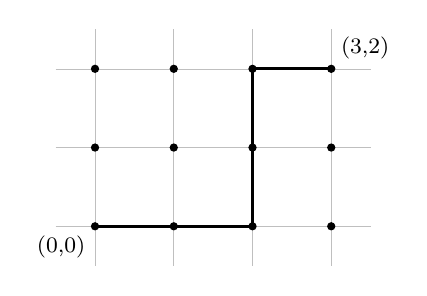
\begin{tikzpicture}
      \draw[very thin, color=gray!50] (-.5,-.5) grid (3.5, 2.5);
      \foreach \x in {0,...,3}
      \foreach \y in {0,...,2}
      \fill (\x,\y) circle (1.5pt);
      \draw (0,0) node[below left] {\footnotesize (0,0)} (3,2) node[above right] {\footnotesize (3,2)};
      \draw[very thick] (0,0) -- (2,0) -- (2,2) -- (3,2);
    \end{tikzpicture}

  \end{center}

  \begin{center}
    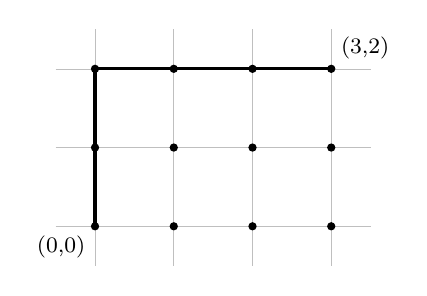
\begin{tikzpicture}
      \draw[very thin, color=gray!50] (-.5,-.5) grid (3.5, 2.5);
      \foreach \x in {0,...,3}
      \foreach \y in {0,...,2}
      \fill (\x,\y) circle (1.5pt);
      \draw (0,0) node[below left] {\footnotesize (0,0)} (3,2) node[above right] {\footnotesize (3,2)};
      \draw[very thick] (0,0) -- (0,2) -- (3,2);
    \end{tikzpicture}

  \end{center}
  
    \begin{center}
    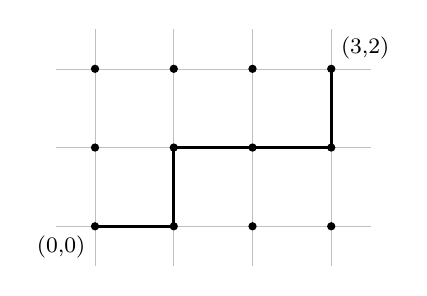
\begin{tikzpicture}
      \draw[very thin, color=gray!50] (-.5,-.5) grid (3.5, 2.5);
      \foreach \x in {0,...,3}
      \foreach \y in {0,...,2}
      \fill (\x,\y) circle (1.5pt);
      \draw (0,0) node[below left] {\footnotesize (0,0)} (3,2) node[above right] {\footnotesize (3,2)};
      \draw[very thick] (0,0) -- (1,0) -- (1,1) -- (3,1) -- (3,2);
    \end{tikzpicture}

  \end{center}
\end{multicols}

Notice that to ensure the path is the {\em shortest} possible, each move must be either to the right or up.  Additionally, in this case, each path has {\em length} 5 - there are a total of 5 steps, each either right or up, which must be taken.

The counting question: how many lattice paths are there between $(0,0)$ and $(3,2)$?  We could try to draw all of these, or instead of drawing them, maybe just list which direction we travel on each of the 5 steps.  One path might be RRUUR, or maybe UURRR, or perhaps RURRU (those correspond to the three paths drawn above).  So how many such strings of R's and U's are there?  

Notice that each of these strings must contain 5 symbols.  Exactly 3 of them must be R's (since our destination is 3 units to the right).  This seems awfully familiar.  In fact, what if we used $1$'s instead of R's and 0's instead of U's?  Then we would just have 5-bit strings of weight 3.  There are 10 of those.  So there are 10 lattice paths from (0,0) to (3,2). 

The correspondence between bit strings and lattice paths does not stop there.  Here is another way to count lattice paths.  Consider the lattice shown below:

  \begin{center}
    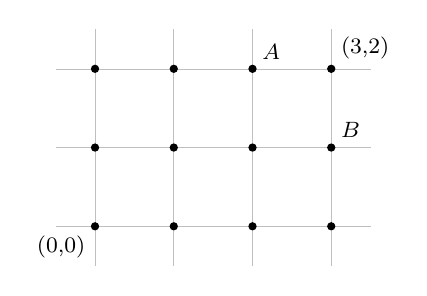
\begin{tikzpicture}
      \draw[very thin, color=gray!50] (-.5,-.5) grid (3.5, 2.5);
      \foreach \x in {0,...,3}
      \foreach \y in {0,...,2}
      \fill (\x,\y) circle (1.5pt);
      \draw (0,0) node[below left] {\footnotesize (0,0)} (3,2) node[above right] {\footnotesize (3,2)};
      \draw (3,1) node[above right] {\footnotesize $B$} (2,2) node[above right]{\footnotesize $A$};
    \end{tikzpicture}

  \end{center}

Now any lattice path from (0,0) to (3,2) must pass through exactly one of $A$ and $B$.  The point $A$ is 4 steps away from (0,0) and two of them are right.  So the number of lattice paths to $A$ is the same as the number of 4-bit strings of weight 2 - that is, 6.  The point $B$ is 4 steps away from (0,0) but now 3 of them are right.  So the number of paths to point $B$ is the same as the number of 4-bit strings of weight 3, namely 4.  So the total number of paths to (3,2) is just $6+4$.  This is the same way we calculated the number of 5-bit strings of weight 3.  The point: exact same recurrence relation exists for bit strings and for lattice paths.


\subsubsection*{Binomial Coefficients}

Binomial coefficients are the coefficients in the expanded version of a binomial such as $(x+y)^5$.  What happens when we multiply such a binomial out?  We will expand $(x+y)^n$ for various values of $n$.  Each of these are done by multiplying everything out (e.g., FOIL-ing) and then collecting like terms.

\[(x+y)^1 = x + y\]
\[(x+y)^2 = x^2 + 2xy + y^2\]
\[(x+y)^3 = x^3 + 3x^2y + 3xy^2 + y^3\]
\[(x+y)^4 = x^4 + 4x^3y + 6x^2y^2 + 4xy^3 + y^4\]

In fact, there is a quicker way to expand the above binomials.  For example, consider the next one, $(x+y)^5$.  What we are really doing is multiplying out,
\[(x+y)(x+y)(x+y)(x+y)(x+y)\]
Now in the expansion, there will be only one $x^5$ term and one $y^5$ term.  That is because to get an $x^5$, we need to use the $x$ term in each of the copies of the binomial $(x+y)$, and similarly for $y^5$.  What about $x^4y$?  To get terms like this, we need to use four $x$'s and one $y$.  So we need exactly one of the five binomials to contribute a $y$.  There are 5 choices for this, so there are 5 ways to get $x^4y$, so the coefficient of $x^4y$ is 5.  This is also the coefficient for $xy^4$ for the same (but opposite) reason - there are 5 ways to pick which of the 5 binomials contribute the single $x$.  So far we have
\[(x+y)^5 = x^5 + 5x^4y + \?x^3y^2 + \?x^2y^3 + 5 xy^4 + y^5\]
We still need the coefficients of $x^3y^2$ and $x^2y^3$.  In both cases, we need to pick exactly 3 of the 5 binomials to contribute one variable, the other two to contribute the other.  Wait.  This sounds familiar.   We have 5 things, each can be one of two things, and we need a total of 3 of one of them.  That's just like taking 5 bits and making sure exactly 3 of them are 1's.  So the coefficient of $x^3y^2$ (and also $x^2y^3$) will be exactly the same as the number of bit strings of length 5 and weight 3, which we found earlier to be 10.  So we have:
\[(x+y)^5 = x^5 + 5x^4y + 10x^3y^2 + 10x^2y^3 + 5 xy^4 + y^5\]

These numbers we keep seeing over and over again - the number of subsets of a particular size, the number of bit strings of a particular weight, the number of lattice paths, and the coefficients of these binomial products - these numbers will all be called {\em binomial coefficients}.  We even have a special symbol for them: ${n \choose k}$.

\begin{defbox}{Binomial Coefficients}
  For each integer $n \ge 0$ and integer $k$ with $0 \le k \le n$ we have a number
  \[{n\choose k}  \]
  read ``$n$ choose $k$.''  We have:
  \begin{itemize}
    \item ${n\choose k} = |\b B^n_k|$, the number of $n$-bit strings of weight $k$.
    \item ${n \choose k}$ is the number of subsets of a set of size $n$ each with cardinality $k$.
    \item ${n \choose k}$ is the number of lattice paths of length $n$ containing $k$ steps to the right.
    \item ${n \choose k}$ is the coefficient of $x^ky^{n-k}$ in the expansion of $(x+y)^n$.
    \item ${n \choose k}$ is the number of ways to select $k$ objects from a total of $n$ objects.
  \end{itemize}
\end{defbox}

The last bullet point is usually taken as the definition of ${n \choose k}$ - we have $n$ objects, and must choose $k$ of them, so there are $n$ choose $k$ ways of doing this.  Each of our counting problems above can be viewed in this way:
\begin{itemize}
  \item How many subsets of $\{1,2,3,4,5\}$ contain exactly 3 elements?  We must choose $3$ of the 5 elements to be in our subset.  There are ${5 \choose 3}$ ways to do this, so there are ${5 \choose 3}$ such subsets.
  \item How many bit strings have length 5 and weight 3?  We must choose $3$ of the 5 bits to be 1's.  There are ${5 \choose 3}$ ways to do this, so there are ${5 \choose 3}$ such bit strings.
  \item How many lattice paths are there from (0,0) to (3,2)?  We must choose 3 of the 5 steps to be towards the right.  There are ${5 \choose 3}$ ways to do this, so there are ${5 \choose 3}$ such paths.
  \item What is the coefficient of $x^3y^2$ in the expansion of $(x+y)^5$?  We must choose 3 of the 5 copies of the binomial to contribute an $x$.  There are ${5 \choose 3}$ ways to do this, so the coefficient is ${5 \choose 3}$.
\end{itemize}

It should be clear that in each case above, we have the right answer.  All we had to do is phrase the question correctly and it became obvious that ${5 \choose 3}$ is correct.  However, this does not tell us that the answer is in fact 10 in each case.  We will eventually find a formula for ${n \choose k}$ but for now, look back at how we arrived at the answer 10 in our counting problems above.  It all came down to bit strings, and we have a recurrence relation for bit strings:
\[|\b B^n_k| = |\b B^{n-1}_{k-1}| + |\b B^{n-1}_k|\]
Remember, this is because we can start the bit string with either a 1 or a 0.  In both cases, we have now have $n-1$ more bits to pick.  The strings starting with 1 must contain $k-1$ more 1's, while the strings starting with 0 still need $k$ more 1's.

Now since $|\b B^n_k| = {n \choose k}$, we can use the same recurrence relation for binomial coefficients:

\begin{defbox}{Recurrence relation for ${n \choose k}$}
  \[{n \choose k} = {n-1 \choose k-1} + {n-1 \choose k}\]
\end{defbox}

\section{Pascal's Triangle}

Let's arrange the binomial coefficients ${n \choose k}$ into a triangle like follows:

\begin{center}
  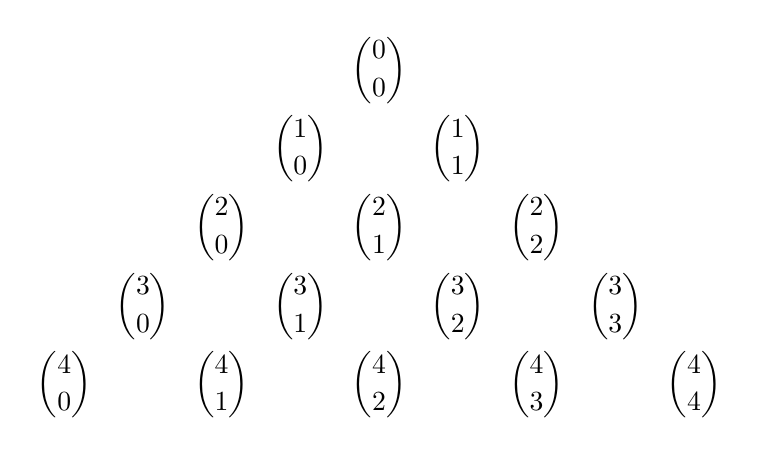
\begin{tikzpicture}
    \foreach \n in {0,...,4}
    \foreach \k in {0,...,\n}
    \draw (-\n+2*\k, -\n) node {$\displaystyle{\n \choose \k}$};
  \end{tikzpicture}

\end{center}

Of course we can continue this as far down as we like.  The recurrence relation for ${n \choose k}$ tells us that each entry in the triangle is the sum of the two entries above it.  The entries on the sides of the triangle are always 1.  This is because ${n \choose 0} = 1$ for all $n$ - there is only one way to pick 0 of $n$ objects - and ${n \choose n} = 1$ since there is one way to select all $n$ out of $n$ objects.  Using the recurrence relation, and the fact that the sides of the triangle are 1's, we can easily replace all the entries above with the correct values of ${n \choose k}$.  Doing so gives us Pascal's triangle.

We can use Pascal's triangle to calculate binomial coefficients.  For example, using the triangle on the next page, we can find ${12 \choose 6} = 924$.

\newpage
\begin{center}
{\Huge Pascal's Triangle}
\vskip 2cm

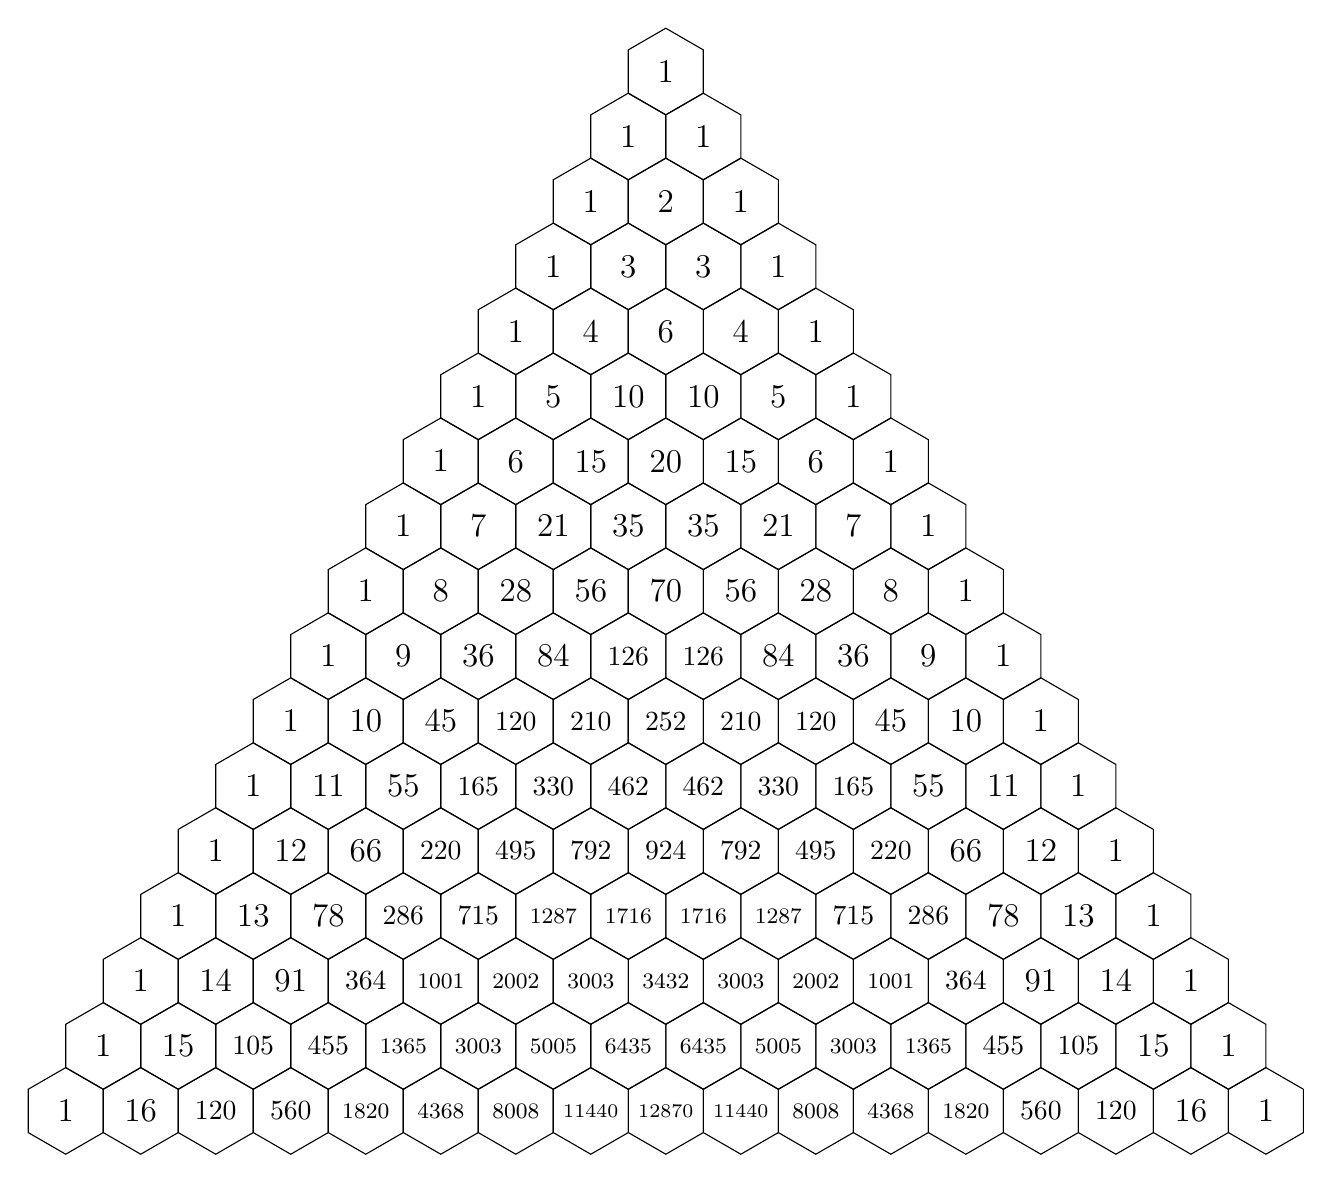
\begin{tikzpicture}
\def\r{.55}
\newcommand{\hexagon}[3]{
  \def\x{-cos{30}*\r*#1+cos{30}*#2*\r*2}
  \def\y{-\r*#1-sin{30}*\r*#1}
  \draw (\x,\y) +(90:\r) -- +(30:\r) -- +(-30:\r) -- +(-90:\r) -- +(-150:\r) -- +(150:\r) -- cycle;
  \draw (\x,\y) node{#3};
}

  
% Pascal's triangle
%put row of 1's down left side:
  \foreach \row in {0,...,16} {
    \hexagon{\row}{0}{\large 1}
  }
%fill in the rest of the triangle:
  \foreach \row in {1,...,16} {
    \pgfmathsetmacro{\entry}{1};
    \foreach \col in {1,...,\row} {
      % iterative formula : val = precval * (row-col+1)/col
      % (+ 0.5 to bypass rounding errors)
      \pgfmathtruncatemacro{\entry}{\entry*((\row-\col+1)/\col)+0.5};
      \global\let\entry=\entry
      \ifnum \entry<100
	\hexagon{\row}{\col}{\large \entry}
      \else \ifnum \entry<1000
	\hexagon{\row}{\col}{\entry}
      \else \ifnum \entry<10000
	\hexagon{\row}{\col}{\footnotesize \entry}
	\else
	\hexagon{\row}{\col}{\scriptsize \entry}
	\fi
      \fi
      \fi
    }
  }
\end{tikzpicture}
\end{center}
\newpage

\section{Combinations and Permutations}

A {\em permutation} is a (possible) rearrangement of objects.  For example, there are 6 permutations of the letters $abc$:
\[abc, ~~ acb, ~~ bac, ~~bca, ~~ cab, ~~ cba\]
We know that we have them all listed above - there are 3 choices for which letter we put first, then 2 choices for which letter comes next, which leaves only 1 choice for the last letter.  The multiplicative principle says we multiply these numbers.

\begin{example}
  How many permutations are there of the letters $abcdef$?
  \begin{solution}
    We do NOT want to try to list all of these out.  However, if we did, we would need to pick a letter to write down first.  There are 6 choices for that letter.  For each choice of first letter, there are 5 choices for the second letter (we cannot repeat the first letter), and for each of those, there are 4 choices for the third, 3 choices for the fourth, 2 choices for the fifth and finally only 1 choice for the last letter.  So there are $6 \cdot 5 \cdot 4 \cdot 3 \cdot 2 \cdot 1 = 720$ permutations of the 6 letters.  We could also write this as $6!$ (that is, 6 factorial).
  \end{solution}
\end{example}

Sometimes we do not want to permute all of the letters. 

\begin{example}
  How many 4 letter ``words'' can you make from the letters a-f, with no repeated letters?
  \begin{solution}
    This is just like the problem of permuting 4 letters.  Only now we have more choices for each letter.  For the first letter, there are 6 choices.  For each of those, there are 5 choices for the second letter.  Then there are 4 choices for the third letter, and 3 choices for the last letter.  The total number of words is $6\cdot 5\cdot 4 \cdot 3 = 360$.  This is not $6!$, but it is almost.  The difference is that in $6!$ we multiply by 2 and 1, where as here we did not.  So to cancel the 2 and 1, we could write $\frac{6!}{2!}$.
  \end{solution}
\end{example}

In general, we can ask how many permutations exist of $k$ objects choosing those objects from a larger $n$-many objects.  (In the example above, $k = 4$, and $n = 6$).  We write this number $P(n,k)$.  From the example above we see that to compute $P(n,k)$ we must apply the multiplicative principle to $k$ numbers, starting with $n$ and counting backwards.  So for example
\[P(10, 4) = 10\cdot 9 \cdot 8 \cdot 7\]
Notice again that $P(10,4)$ starts out looking like $10!$, but we stop after 7.  So
\[P(10,4) = \frac{10\cdot 9 \cdot 8 \cdot 7 \cdot 6 \cdot 5 \cdot 4 \cdot 3 \cdot 2 \cdot 1}{6 \cdot 5 \cdot 4 \cdot 3 \cdot 2 \cdot 1} = \frac{10!}{6!}\]
Careful - the factorial in the denominator is not $4!$ but rather $(10-4)!$.  

\begin{defbox}{Permutations}
 $P(n,k)$ is the number of permutations of $k$ out of $n$ objects.
 
 \[P(n,k) = \frac{n!}{(n-k)!}\]
\end{defbox}

Note that when $n = k$, we have $P(n,n) = \frac{n!}{(n-n)!} = n!$ (since $0! = 1$).  This makes sense - we already had that $n!$ gives the number of permutations of all $n$ objects.

Here is another way to find the number of permutations of $k$ out of $n$ objects: first select which $k$ objects will be in the permutation, then count how many ways there are to arrange them.  Once you have selected the $k$ objects, we know there are $k!$ ways to arrange (permute) them.  But how do you select $k$ objects from the $n$?  You have $n$ objects, and you need to {\em choose} $k$ of them.  You can do that in ${n \choose k}$ ways.  This says:
\[P(n,k) = {n \choose k}\cdot k!\]

Now since we have a closed formula for $P(n,k)$ already, we can substitute that in:
\[\frac{n!}{(n-k)!} = {n \choose k} \cdot k!\]
If we divide both sides by $k!$ we get a closed formula for ${n \choose k}$.

\begin{defbox}{Closed formula for ${n \choose k}$}
  \[{n \choose k} = \frac{n!}{(n-k)!k!}\]
\end{defbox}

We say $P(n,k)$ counts permutations, and ${n \choose k}$ counts {\em combinations}.  The formulas for each are very similar - there is just an extra $k!$ in the denominator of ${n \choose k}$.  That extra $k!$ accounts for the fact that ${n \choose k}$ does not distinguish between the different orders that the $k$ objects can appear in - we are just selecting (or choosing) the $k$ objects, not arranging them.  Perhaps ``combination'' is a misleading label - we don't mean it like a combination lock (where the order would definitely matter).  Perhaps better: a combination of flavors - you just need to decide which flavors to combine, not the order in which to combine them.

To further illustrate the connection between combinations and permutations, we close with an example.

\begin{example}
  You decide to have a dinner party.  Even though you are incredibly popular and have 14 different friends, you only have enough chairs to invite 6 of them.  
  \begin{enumerate}
    \item How many choices do you have for which 6 friends to invite? 
    \item What if you need to decide not only which friends to invite but also in which order to invite them in?  How many choices do you have then?
  \end{enumerate}
  \begin{solution}
    \begin{enumerate}

      \item You must simply choose 6 friends from a group of 14.  This can be done in ${14 \choose 4}$ ways.  We can find this number either by using Pascal's triangle or the closed formula $\frac{14!}{8!\cdot 6!} = 3003$.
      
      \item Here you must count all the ways you can permute 6 friends chosen from a group of 14.  So the answer is $P(14, 6)$, which can be calculated as $\frac{14!}{8!} = 2192190$
   \end{enumerate}
    How are these numbers related?  Notice that $P(14,6)$ is {\em much} larger than ${14 \choose 6}$.  This makes sense - ${14 \choose 6}$ picks 6 friends, but $P(14,6)$  arranges them the 6 friends as well as picks them.  In fact, we can say exactly how much larger $P(14,6)$ is.  In both counting problems we choose 6 out of 14 friends.  For the first one, we stop there - at 3003 ways.  But for the second counting problem, each of those 3003 choices of 6 friends can be arranged in exactly $6!$ ways.  So now we have $3003\cdot 6!$ choices - and that is exactly $2192190$.
    
    Alternatively, look at the first problem another way.  We want to select 6 out of 14 friends, but we do not care about the order they are selected in.  To select 6 out of 14 friends, we might try this:
    \[14 \cdot 13 \cdot 12 \cdot 11 \cdot 10 \cdot 9\]
    This is a reasonable guess, since we have 14 choices for the first guest, then 13 for the second, and so on.  But the guess is wrong (in fact, that product is exactly $2192190 = P(14,6)$).  It distinguishes between the different orders in which we could invite the guests.  To correct for this, we could divide by the number of different arrangements of the 6 guests (so that all of these would count as just one outcome).  There are precisely $6!$ ways to arrange 6 guests, so the correct answer to the first question is
    \[\frac{14 \cdot 13 \cdot 12 \cdot 11\cdot 10 \cdot 9}{6!}\]
    Note that another way to write this is
    \[\frac{14!}{8!\cdot 6!}\]
    which is what we had originally.
  \end{solution}

\end{example}



\end{document}


